\documentclass{amsart}
\usepackage{graphicx}
\graphicspath{{./}}
\usepackage{hyperref}
\usepackage{csvsimple}
\usepackage{longtable}
\usepackage{lscape}
\usepackage{epigraph}
\title{Ethnicity Effects on Human Race Child-Rearing Values} 
\author{Zulfikar Moinuddin Ahmed}
\date{\today}
\begin{document}
\maketitle
\epigraph{My entire ouvre of Quantitative Human Nature is dedicated as a Labour of Love to my Beloved People, the Human Race.}{Allen, Texas, May 24 2021}

\section{Summary of Results}

We consider analysis of 11 questions related to human race child-rearing moral values.  They are questions 7 through 17 of World Values Survey.  Our main finding is that the Ethnicity effect on these values roughly explain 9.52\% of the total variation.  

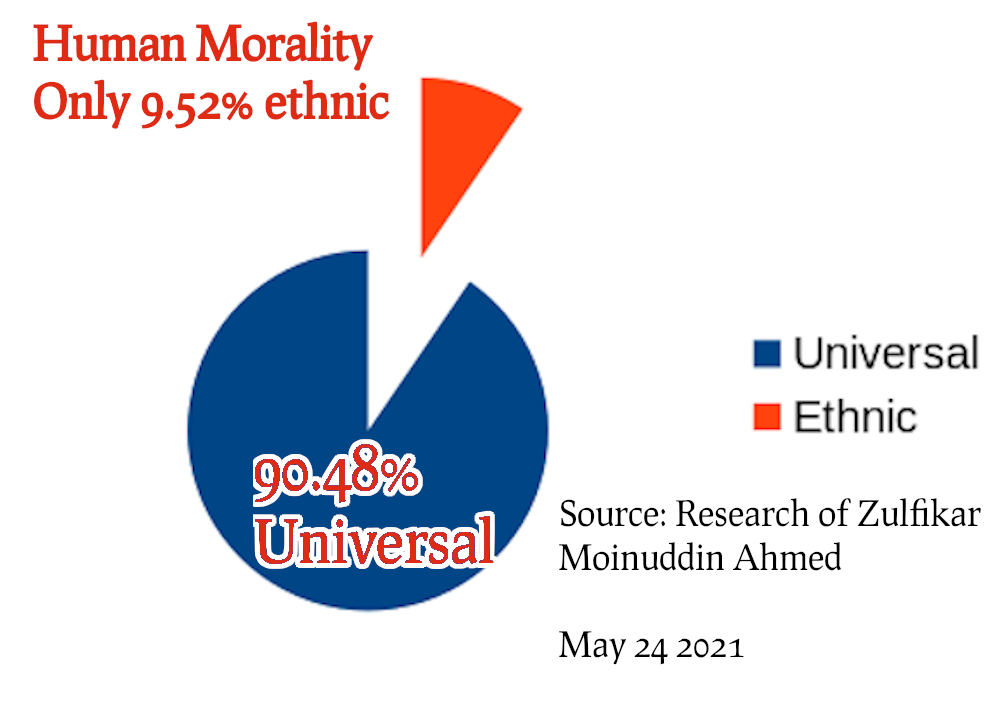
\includegraphics[angle=180,scale=-.3]{ethnic_slice.png}

This is the outcome of a fair amount of sophisticated work.  We will start at the end of the journey.  This is the table of dispersion of estimate Bernoulli $p$-value for each question across six ethnicity classes.  The total sample is $N=19077$.

% latex table generated in R 4.0.3 by xtable 1.8-4 package
% Mon May 24 11:32:51 2021
\begin{table}[ht]
\centering
\begin{tabular}{rlr}
  \hline
 & q & bernoulli.p.sigma \\ 
  \hline
1 & Q7 & 0.0942 \\ 
  2 & Q8 & 0.1250 \\ 
  3 & Q9 & 0.1467 \\ 
  4 & Q10 & 0.0539 \\ 
  5 & Q11 & 0.0405 \\ 
  6 & Q12 & 0.0589 \\ 
  7 & Q13 & 0.0870 \\ 
  8 & Q14 & 0.0961 \\ 
  9 & Q15 & 0.1411 \\ 
  10 & Q16 & 0.0955 \\ 
  11 & Q17 & 0.1084 \\ 
   \hline
\end{tabular}
\end{table}

We will strive to ensure that the public is able to reproduce these numbers themselves.  Our data source was World Values Survey, Wave 7.  The interested reader can use open source R and packages to reproduce our results for their own pleasure.

\section{Bernoulli $p$ Table}

The summary per question in the last section are the row-wise standard deviation of the following table, with ethnicity as the columns.  

These are Bernoulli $p$ parameter estimates.  This the outcome of a fairly complex process, and form the basis of our conclusion regarding ethnicity effects of the child-rearing moral values of the human race.  The rest of this note will address how we came to these figures.  A previous note of mine used sample frequency as the Bernoulli $p$-parameter.  We had concluded an estimate that ethnicity explains 13.9\% of the variation in child-rearing moral values of the human race.  Here we constrain the value further to 9.52\% based on much more sophisticated statistical techniques.

% latex table generated in R 4.0.3 by xtable 1.8-4 package
% Mon May 24 12:15:01 2021
\begin{table}[ht]
\centering
\begin{tabular}{rrrrrrr}
  \hline
 & Arab & Black & East Asian & Indian & Other & White \\ 
  \hline
Q7 & 0.843 & 0.680 & 0.746 & 0.786 & 0.737 & 0.787 \\ 
  Q8 & 1.000 & 0.778 & 1.000 & 0.836 & 0.723 & 0.763 \\ 
  Q9 & 1.000 & 0.778 & 0.709 & 0.770 & 1.000 & 1.000 \\ 
  Q10 & 0.728 & 0.738 & 0.804 & 0.817 & 0.758 & 0.789 \\ 
  Q11 & 0.743 & 0.758 & 0.772 & 0.860 & 0.795 & 0.783 \\ 
  Q12 & 0.752 & 0.776 & 0.715 & 0.882 & 0.760 & 0.733 \\ 
  Q13 & 1.000 & 0.797 & 0.799 & 0.818 & 0.810 & 0.815 \\ 
  Q14 & 1.000 & 0.887 & 0.750 & 0.883 & 0.800 & 0.729 \\ 
  Q15 & 1.000 & 0.739 & 0.711 & 1.000 & 0.725 & 0.789 \\ 
  Q16 & 0.759 & 1.000 & 1.000 & 1.000 & 1.000 & 1.000 \\ 
  Q17 & 0.800 & 1.000 & 1.000 & 1.000 & 1.000 & 1.000 \\ 
   \hline
\end{tabular}
\end{table}

The final result of 9.52\% variation arises from the mean of the row-wise standard deviations of this table.

\section{Connection to Markov Moral Model}

My earlier work on Markov Chains to model moral value distribution was not based on the variables Q7-Q17 but on others in World Values Survey.  These other moral variables were measures in scale of 1-10.  The measurements of Q7-Q17, by contrast are binary.  The main connection is that I had found that my Markov Moral Model explained 91\% of the variation of the human race moral values.  We distinguish Q7-Q17 by calling these 'child-rearing moral values'.   It is gratifying to see that 9.52\% arises in these cases as being explained by ethnicity.  This allows us to have greater confidence of our decomposition of effect of {\em universal human nature} to be roughly 91\% and ethnicity effects to be around 9\%.  We expect these to remain roughly the same for thousands of years to come, maybe shrink a bit or expand a bit.  The intuition here is that these depend on evolutionary time.  We will not establish this intuition, but our race, the human race, has been out of Africa for around 75,000 years.  Our evolution for around $75,000 \times 9 = 675,000$ years before this exodus from East Africa, we have developed basis for our moral nature.  So this is quite good a rule of thumb for me, to expect that our morals are 91\% universal and 9\% ethnicity-specific. 


Let me give you the list directly for association and calibration to ordinary reality.

% latex table generated in R 4.0.3 by xtable 1.8-4 package
% Mon May 24 14:17:44 2021
\begin{table}[ht]
\centering
\begin{tabular}{rll}
  \hline
 & vars & chdesc \\ 
  \hline
1 & Q7 & good manners \\ 
  2 & Q8 & independence \\ 
  3 & Q9 & hard work \\ 
  4 & Q10 & feeling of responsibility \\ 
  5 & Q11 & imagination \\ 
  6 & Q12 & tolerance and respect for others \\ 
  7 & Q13 & thrift saving money \\ 
  8 & Q14 & perserverence \\ 
  9 & Q15 & religious faith \\ 
  10 & Q16 & unselfishness \\ 
  11 & Q17 & obedience \\ 
   \hline
\end{tabular}
\end{table}

We will not delve into sociological issues here.  We keep focus on how ethnicity as a variable affects the distribution of these variables at a purely statistical level.  Our main focus is on ensuring that the statistical inference scheme is strongly justified scientifically.  My background is Mathematics and I am responsible for Four-Sphere Physics theory and have many years of experience as a Finance Quant.  As a result, I am far more concerned with issues of how statistical models actually match inscrutible Nature rather than interpretations that are humanistic.  The final inference is of course that all theories of moral superiority on ethnic grounds are impossible since only 9.52\% of human (childrearing) values are affected by ethnicity at all, and it is implausible to produce any meaningful 'moral superiority' with 9.52\% of variation.  And since 'racial superiority' theories have a necessary moral component, we refute all such theories everywhere on Earth and not just in America and Europe.

\section{The Actual Code}

I will go through the path that led to the strong statistical fits of particular models.  Before I do that, I want to ensure that people interested in having a hands on experience with the actual data have the ability to get the data.  

Our data comes from the spectacularly high quality data collected from hundreds of thousands of people around the world by World Values Survey. Wave 7 has an RDS file with data that I use \cite{WVS}.

\begin{verbatim}
# load data
wvs7<-readRDS("wvs7.rds")
vars<-c("Q1","Q2","Q3","Q4","Q5","Q6",
        "Q7","Q8","Q9","Q10", "Q11",
        "Q12", "Q13", "Q14", "Q15", "Q16", "Q17",
        "Q290","Q46", "Q177","Q178","Q179","Q180","Q181","Q182","Q183","Q184","Q185","Q186","Q187","Q188","Q189","Q190","Q191","Q192","Q193","Q194","Q195","Q275",
        "Q192","Q199", "Q57", "Q58", "Q59", "Q60", "Q61", "Q62",
        "Q63","Q64","Q65","Q66","Q67","Q68","Q69",
        "Q70","Q71","Q72","Q73","Q74","Q75","Q76","Q77","Q78",
        "Q79","Q80", "Q81", "Q82", "Q83","Q84","Q85","Q86","Q87",
        "Q88","Q89","Q90", 
        "Q235", "Q236", "Q237", "Q238", "Q239","Q240",
        "Q241", "Q242",
        "Q253", "Q254","Q255","Q256","Q257", "Q258","Q259", 
        "Q260")

# Create ethnicity table 
# by mapping various detailed
# country-based ethnicities to
# broader groups
library(haven)
# Problem is WVS Q290 has too many 
# gradations when we want to deal 
# with a few classes that can allow 
# us to overcome ethnic prejudices
ethnicities<-unique(as.character(as_factor(wvs7$Q290)))

reduced_ethnicities<-function(){
  mapeth<-rep("Other",length(ethnicities))
  mapeth[c(1,7,15,33,38,43,65,107,154,210,214)]<-"White"
  mapeth[c(3,223,222,51,52,53,54,55,56,45,39,36,11)]<-"Black"
  mapeth[c(6,13,19,20,21,22,67,70)]<-"Indian"
  mapeth[c(4,17,48,97,98,99,100)]<-"Arab"
  mapeth[c(5,14,16,62,63,64,68,72,73,74,75,76,77,
           78,79,80,81,82,83)]<-"East Asian"
  data.frame(key=ethnicities,val=mapeth)
}

ethnicity_map<-function( v ){
  emap<-reduced_ethnicities()
  w<-sapply(as.character(as_factor(v)),function(x) { out<-emap[which(emap$key==x),]$val; if(is.null(out)){out<-"Other"};return(out)})
  #print(head(w))
  #w<-append(w,"Other")
  as.factor(unlist(w))
}



polv<-na.omit(wvs7[,vars])
polv$eth<-ethnicity_map(as_factor(polv$Q290))

# We will use logistic regression
# with x variable artificially created for Q7-Q17
# We take N=500 points to determine p, lambda
# Then we use these to assign random x values
# for all the other values
# then we fit logistic regression on the (x,g)

chdesc<-c("good manners", "independence", "hard work",
          "feeling of responsibility", "imagination", 
          "tolerance and respect for others", "thrift saving money",
          "perserverence","religious faith", "unselfishness","obedience")

samp.binary.exp<-function( grps, lambda ){
  grps<-as.vector(t(grps))
  n <- length(grps)
  print(n)
  gvals <- unique(grps)
  #print(gvals)
  bval <- 0
  sval <- 1
  if ( length(gvals) == 2 ){
    if ( sum(gvals==gvals[1]) >= n/2 ){
      bval <- gvals[1]
      sval <- gvals[2]
    } else {
      sval <- gvals[1]
      bval <- gvals[2]
    }
  } else {
    return(NULL)
  }
  xs<- rep( 0, n)
  for ( r in 1:n ){
    done <- F
    
    while ( done == F){
      pickx <- rexp(1,rate=1/lambda)
      #print(pickx)
      if (pickx <= log(2)/lambda){
        if ( grps[r] == sval){
          xs[r] <- pickx
          done <- T
        }  
      }
      if (pickx > log(2)/lambda){
        if ( grps[r] == bval){
          xs[r] <- pickx
          done <- T
        }  
      }
    }
  }
  xs
}

dataset.logit<-function(var,lambda){
  y<-na.omit(polv[,var])
  G<-as.numeric(as_factor(t(y)))-1
  p<-sum(G==0)/length(G)
  if ( p < 0.5) {
    G<-1-G
  }
  p<-sum(G==0)/length(G)
  print(p)
  
  x<-samp.binary.exp( G, lambda)
  out<-data.frame( x=x,G=G)
  names(out) <- c("x","G")
  out
}

dataset.logit.fixed.lambda<-function(var){
  y<-na.omit(polv[,var])
  G<-as.numeric(as_factor(t(y)))-1
  p<-sum(G==0)/length(G)
  if ( p < 0.5) {
    G<-1-G
  }
  p<-sum(G==0)/length(G)
  print(p)
  lambda <- 2*log( p/(1-p) )
  #print(head(y))
  x<-samp.binary.exp( y, max(lambda,2.4))
  out<-data.frame( x=x,G=G)
  names(out) <- c("x","G")
  out
}

if (FALSE){
lq14<-dataset.logit.fixed.lambda("Q14")
mq14 = glm( G ~ x, family="binomial",data=lq14)
summary(mq14)
}



dataset.logit.eth<-function(var,eth){
  y0<-na.omit(polv[,var])
  G0<-as.numeric(as_factor(t(y0)))-1
  p0<-sum(G0==0)/length(G0)
  if ( p0 < 0.5) {
    G0<-1-G0
  }
  p0<-sum(G0==0)/length(G0)
  lambda0 <- 2*log( p0/(1-p0) )
  #lambda <- max(min(lambda,2.7),1.5)
  lambda0 <- max(lambda0,2)
  #print(head(y))
  x0<-samp.binary.exp( y0, lambda0)
  
  idx<-as.character(polv$eth)==eth
  y<-na.omit(polv[idx,var])
  G<-as.numeric(as_factor(t(y)))-1
  x<-x0[idx]
  p<-sum(G==0)/length(G)
  if ( p < 0.5) {
    G<-1-G
  }
  p<-sum(G==0)/length(G)
  #print(p)
  lambda <- 2*log( p/(1-p) )
  out<-data.frame( x=x,G=G)
  names(out) <- c("x","G")
  list(df=out,lambda=lambda)
}

dataset.logit.eth2<-function(var,eth){
  y<-na.omit(polv[as.character(polv$eth)==eth,var])
  G<-as.numeric(as_factor(t(y)))-1
  p<-sum(G==0)/length(G)
  if ( p < 0.5) {
    G<-1-G
  }
  p<-sum(G==0)/length(G)
  print(p)
  lambda <- 2*log( p/(1-p) )
  #lambda <- max(min(lambda,2.7),1.5)
  lambda <- min(max(lambda,0.3),2)
  #print(head(y))
  x<-samp.binary.exp( y, lambda)
  out<-data.frame( x=x,G=G)
  names(out) <- c("x","G")
  list(df=out,lambda=lambda)
}

vars<-c("Q7","Q8","Q9","Q10","Q11","Q12",
        "Q13","Q14","Q15","Q16","Q17")

eths<-c("Arab", "Black","East Asian", "Indian", "Other", "White")

child.eth<-function(){
  lambdas <- matrix( 0, nrow=length(vars), ncol=length(eths))
  alphas <- matrix( 0, nrow=length(vars), ncol=length(eths))
  pvals <- matrix( 0, nrow=length(vars), ncol=length(eths))
  bdf <- data.frame()
  for (r in 1:length(vars)){
    for (s in 1:length(eths)){
      A<-dataset.logit.eth( vars[r], eths[s])
      m <- glm( G ~ x, family="poisson", data=A$df)
      lambdas[r,s]<-A$lambda
      alphas[r,s]<-summary(m)$coefficients[2,1]
      pvals[r,s]<-summary(m)$coefficients[2,4]
      bdf<-rbind(bdf,c(vars[r],eths[s],alphas[r,s],lambdas[r,s],pvals[r,s]))
    }
  } 
  names(bdf)<-c("var","eth","alpha","lambda","pval")
  list(df=bdf,lambda=lambdas,alpha=alphas,pvals=pvals)
}
\end{verbatim}

\section{Our Approach}

Our approach to dealing with Bernoulli data is to simulate $x$ data from the exponential distribution with our data $g$ as labels appropriately. We were originally interested in Generalised Linear Models with logit link.  We found success with Poisson regression with log link instead.  

All $p$ Values of the Poisson regression for all Ethnicities are lower than $1e-16$ in our fits.  Our scheme provides extremely good fit to the data. 

See the actual code for details.

\section{Closer Look At Estimated Coefficients From Poisson Regression}

% latex table generated in R 4.0.3 by xtable 1.8-4 package
% Mon May 24 17:11:12 2021
\begin{table}[ht]
\centering
\begin{tabular}{rrrrrrr}
  \hline
 & Arab & Black & East Asian & Indian & Other & White \\ 
  \hline
good manners & 1.2782 & 0.2931 & 0.2526 & 0.9424 & 0.2200 & 0.2652 \\ 
  independence & -4.0733 & 0.3211 & -3.5651 & 0.2924 & 0.1990 & 0.2000 \\ 
  hard work & -5.0535 & 0.2621 & 0.2060 & 0.2570 & -3.4818 & -3.3346 \\ 
  feeling of responsibility & 0.3891 & 0.2490 & 0.3290 & 0.3911 & 0.2461 & 0.2773 \\ 
  imagination & 0.1864 & 0.2427 & 0.2096 & 0.2932 & 0.2437 & 0.2631 \\ 
  tolerance and respect for others & 0.4222 & 0.3365 & 0.2045 & 0.1959 & 0.2322 & 0.2420 \\ 
  thrift saving money & -3.9867 & 0.4465 & 0.2553 & 0.3158 & 0.2598 & 0.2782 \\ 
  perserverence & -3.7042 & 0.3876 & 0.2630 & 0.4453 & 0.2704 & 0.2532 \\ 
  religious faith & -4.9020 & 0.2174 & 0.2115 & -5.0846 & 0.1973 & 0.2685 \\ 
  unselfishness & 0.1844 & -4.8956 & -6.5116 & -4.2878 & -4.7394 & -4.7288 \\ 
  obedience & 0.3187 & -3.4906 & -5.0112 & -5.7486 & -3.9494 & -3.7205 \\ 
   \hline
\end{tabular}
\end{table}

Our approach is to produce a synthetic $x$ vector based on the whole data and then subsetting the appropriate points for each ethnicity.  



\begin{thebibliography}{CCC}
\bibitem{WVS}{\url{}}
\end{thebibliography}
\end{document}